\documentclass[11pt]{beamer}
\title{Learning Nonlinear Loop Invariant with Gated Continuous Logic Networks}
\usepackage{verbatim}
\usepackage{amsmath}
\usepackage{amsthm}
\usepackage{graphics}
\usepackage{color}
\usepackage{stmaryrd}
\usepackage{multicol}

\newtheorem{proposition}{Proposition}

\date{\today}
\author{Jianan Yao et. al}


\begin{document}
\maketitle

\begin{frame}\frametitle{History of the Research}

\begin{center}
\textsc{CLN2INV: Learning Loop Invariants with Continuous Logic Networks}
\end{center}

In this paper, they propose the algorithm of learning loop invariants using CLN.

This paper generalize the model into GCLN, where ``G'' stands for gated.

\end{frame}
\begin{frame}\frametitle{Overview}
\begin{itemize}
\item Introduction to learning nonlinear invariant.
\item Workflow of the algorithm.
\item Detailed description of the theory and techniques.
\item Experimental evaluation.
\end{itemize}

\end{frame}
\begin{frame}\frametitle{Difficulties}
\begin{itemize}
\item Large search space with high magnitude terms. e.g. terms like $x^2$ and $x^y$ grows exponentially.

\item Limitted samples. Bounds on the number of loop iterations with integer variables.

\item Distinguishing sufficient inequalities.

\end{itemize}

\end{frame}

\begin{frame}\frametitle{Ways to Resolve}
\begin{itemize}

\item \textbf{Learning with G-CLNs}, where the gated value can be used to turn on or off the terms. Combine dropout.(Example)

\item \textbf{Fractional sampling}. Relax the semantic of the loop to continuous functions.

\item \textbf{Piecewise Biased Quadratic Units(PBQU)}. A way to penalizes loose fits and converges to tight contraints on data.(Example)

\end{itemize}
\end{frame}
\begin{frame}\frametitle{Background}
\begin{definition}[Loop Invariant Inference]
Given the precondition $P$ and postcondition $Q$. Finding an inductive invariant $I$ such that,

\[P\Longrightarrow I, \{I\wedge LC\}C\{I\}, I\wedge \neg LC \Longrightarrow Q\]

\end{definition}
Loop invariants can be encoded in SMT. The data driven invariant inference is to find SMT formula $F$ s.t.
\[\forall x\in X, F(x) = True\]


\end{frame}

\begin{frame}\frametitle{Making Loop Invariant Learnable}
Using a differentiable logic: Basic Fuzzy Logic(BL). BL is a relaxation of FOL on continuous truth value on the interval $[0,1]$.

\begin{itemize}
\item t-norms($\otimes$). Consistency: $t \otimes 1 = 1, t \otimes 0 = 0$, commutative and monotonic.

\item t-conorms($\oplus$), operates as disjunctions for BL and derived from DeMorgan's law with $\neg t = 1 - t$ 
\end{itemize}




\end{frame}

\begin{frame}\frametitle{Semantic Mapping}
Principles:
\begin{enumerate}
\item Remain the meaning of the logic.
\item Continuous and smooth.
\item Increasing when unsat terms change to sat terms.
\end{enumerate}
We use $\mathcal{S}$ as the mapping function and it is defined recursively. $\mathcal{S}(F) : X \rightarrow [0,1]$.
\begin{center}
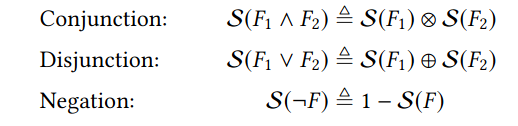
\includegraphics[scale=0.4]{2.png}

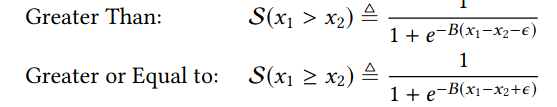
\includegraphics[scale=0.4]{3.png}
\end{center}
\end{frame}

\begin{frame}\frametitle{Example}
\begin{center}
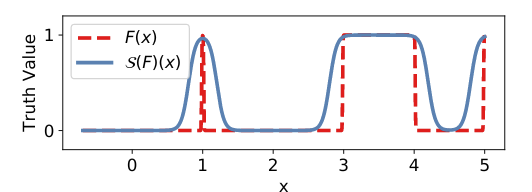
\includegraphics[scale=0.5]{4.png}
\end{center}
\end{frame}
\begin{frame}\frametitle{Workflow}
\begin{center}
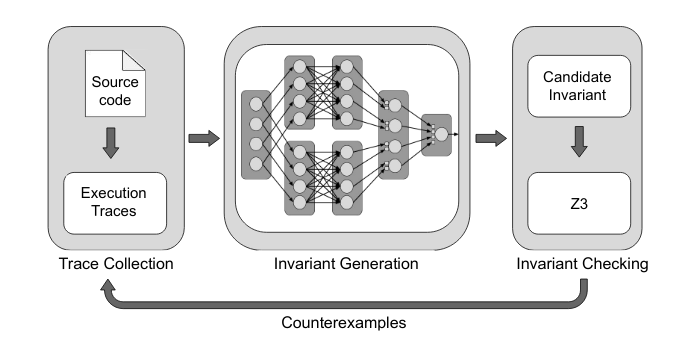
\includegraphics[scale=0.45]{5.png}
\end{center}


\end{frame}

\begin{frame}\frametitle{Continuous Logic Network}
\begin{example}
\begin{center}
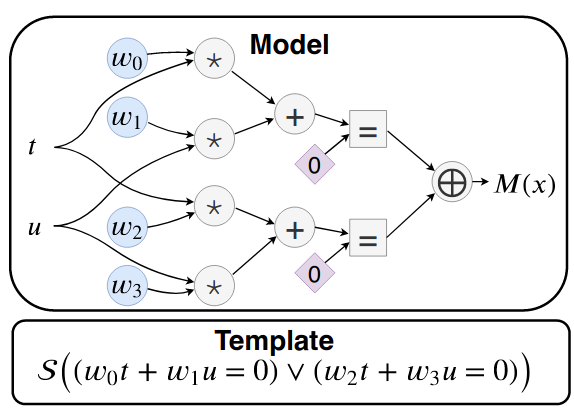
\includegraphics[scale=0.4]{1.png}
\end{center}
\end{example}
\end{frame}

\begin{frame}\frametitle{Gated Continuous Logic Network}
Previous invariant learning with CLN require a preset template. To let the model fit the data automatically instead of given a template ahead, we use gated CLN.

gated t-norms:
\[T_G(x,y;g_1,g_2) = (1 + g_1(x - 1))\otimes (1 + g_2(y - 1)) \]
Likewise for gated t-conorms.

\begin{center}
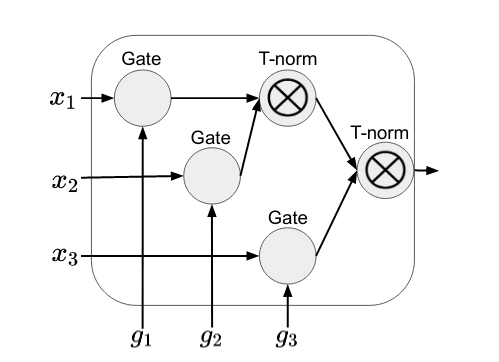
\includegraphics[scale=0.35]{7.png}
\end{center}
Current learning parameters: $W, g_i$
\end{frame}
\begin{frame}\frametitle{Learning Target}
Minimize
\[\mathcal{L}(X; W,G) = \sum_{x\in X}(1 - \mathcal{M}(x; W,G)) + \lambda_1\sum_{g_1\in T_G}(1 - g_i) + \lambda_2 \sum_{g_i\in T_G' }g_i\]
where $\lambda_i$ are normalization parameters.
\end{frame}


\begin{frame}\frametitle{Formula Extractions}
\begin{center}
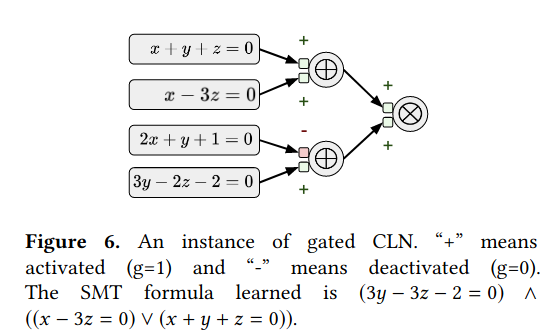
\includegraphics[scale=0.5]{6.png}
\end{center}
\end{frame}
\begin{frame}\frametitle{Formula Extractions}
\begin{center}
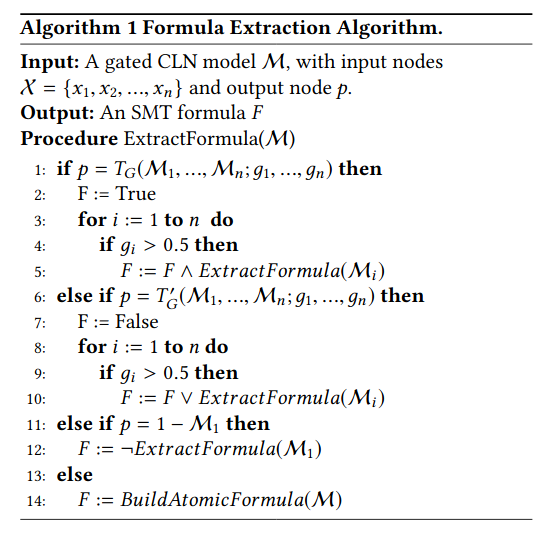
\includegraphics[scale=0.4]{8.png}
\end{center}
\end{frame}


\begin{frame}\frametitle{Piecewise Construction}
\begin{center}
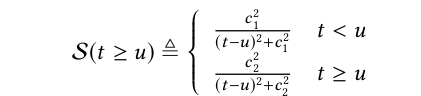
\includegraphics[scale=0.5]{9.png}

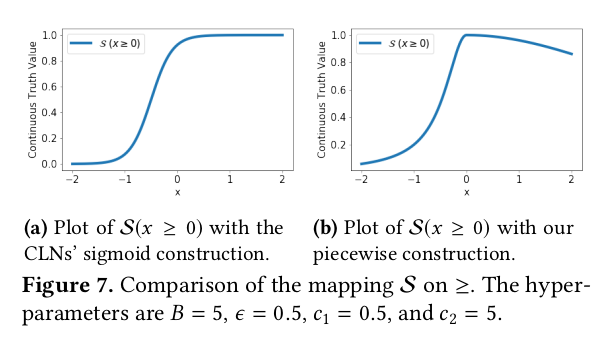
\includegraphics[scale=0.4]{10.png}
\end{center}


\end{frame}

\begin{frame}\frametitle{Fractional Sampling}
\begin{center}
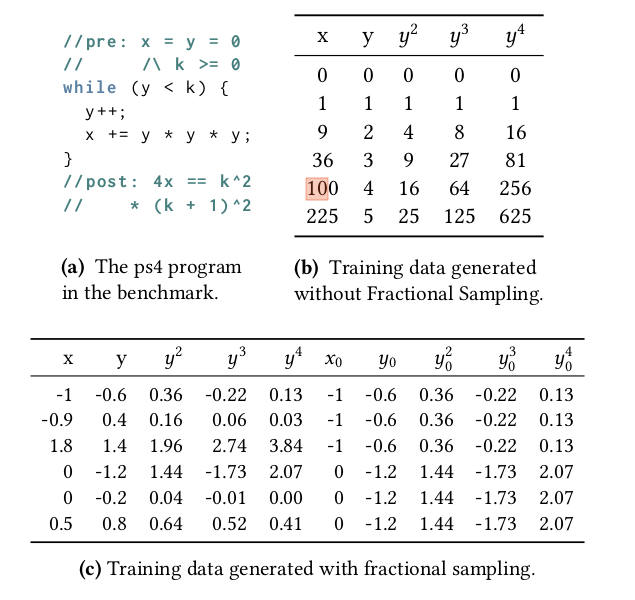
\includegraphics[scale=0.4]{11.png}
\end{center}
\end{frame}

\begin{frame}\frametitle{Optimization}
\textbf{Data Normalization:}

Large inputs cause instability and prevent the CLN model from converging. In the implementation, the paper requires the L2-norm equals a set value $l$.

\textbf{Weight Regularization}

To avoid trivial invariant, we require the $L^p$-norm of the weight vector equals to a nonzero value.

\textbf{Term Dropout:}

Large number of terms poses diffuculties for learning. Random dropout of terms.

\end{frame}

\begin{frame}\frametitle{Experimental Evaluation: Nonlinear}
\begin{center}
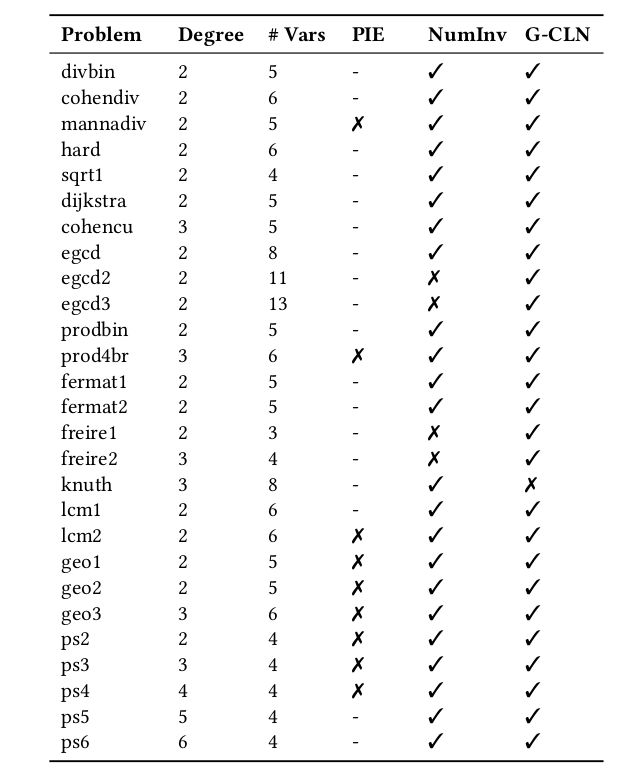
\includegraphics[scale=0.3]{12.png}
\end{center}
\end{frame}

\begin{frame}\frametitle{Experimental Evaluation: Nonlinear}
\begin{center}
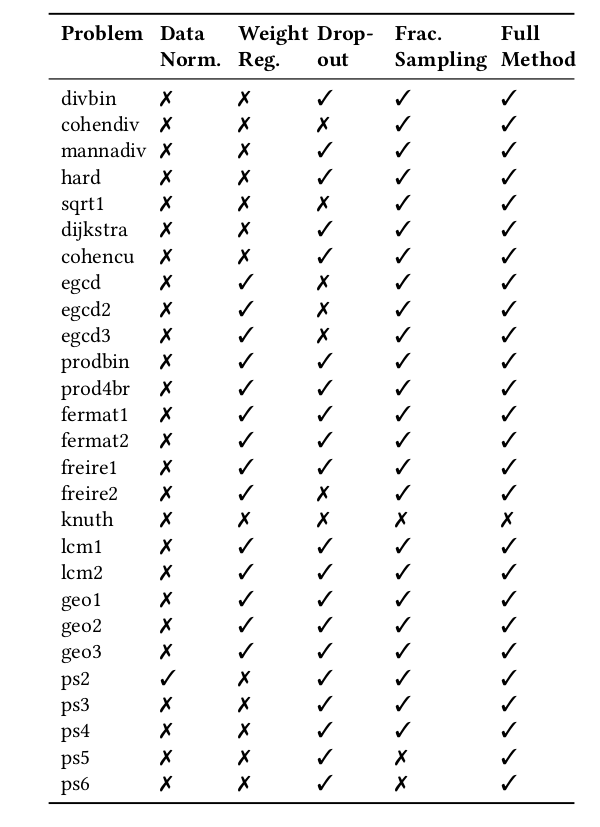
\includegraphics[scale=0.3]{13.png}
\end{center}
\end{frame}

\begin{frame}\frametitle{Experimental Evaluation: Nonlinear}
\begin{center}
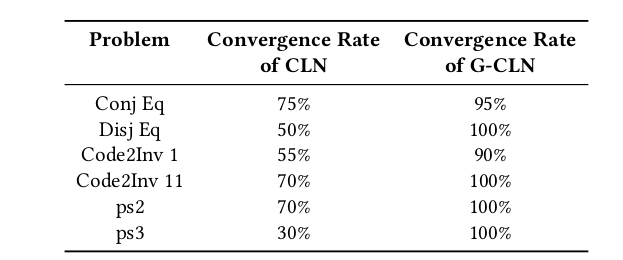
\includegraphics[scale=0.3]{14.png}
\end{center}
\end{frame}

\begin{frame}\frametitle{Experimental Evaluation: Linear}
Among 133 linear cases, except 9 unsovable cases, the tool solved all of the rest.
\end{frame}
\end{document}